\documentclass[12pt]{article}

\usepackage[
%	top=20mm,
%	bottom=20mm,
%	left=20mm,
%	right=20mm,
%	includehead
a4paper,
%scale={0.8,0.5},
%includeheadfoot,
includefoot,
ignoremp,
%ignorefoot,
layouthoffset=0pt,
top=3.5cm,
bottom=1.25cm,
footskip=1.25cm,
headsep=2cm,
scale=0.7,ignorehead,
headheight=21pt
%showframe
]{geometry}
\usepackage{array}
\usepackage{graphicx}
\usepackage{color}

%\includegraphics[height=3cm]{example-image.pdf}%
%\usepackage{bbm}
\usepackage{testpackage}
\usepackage{pgfplots}
\setromanfont{Fira Sans}
\setmainfont{Fira Sans}
\everymath\expandafter{\the\everymath\rm}
\everydisplay\expandafter{\the\everydisplay\rm}
\pagestyle{fancy}
\fancyheadoffset[]{50pt}
\lhead{\rule{\linewidth}{2pt}\\ \hspace{1cm} }
% \lhead{Δημήτρης Τσορτανίδης}
\chead{ΔΗΜΗΤΡΗΣ ΤΣΟΡΤΑΝΙΔΗΣ ΜΑΘΗΜΑΤΙΚΟΣ MSc}
\rhead{2018}
%\setlength{\textwidth}{0.6\paperwidth} 

\usepackage{xgreek}
\usepackage{setspace}
\usepackage{pdfpages}
\renewcommand{\baselinestretch}{1.5} 
% =============================================
  \DeclareSymbolFont{AMSb}{U}{msb}{m}{n}
  \DeclareSymbolFontAlphabet{\mathbb}{AMSb} %επιτρέπει τη χρήση του mathbb https://tex.stackexchange.com/questions/22043/how-to-get-the-ams-mathbb-font-while-using-palatino-elsewhere
% =============================================
\begin{document}
%		\tableofcontents
%		\listoffigures
%		\listoftables
\begin{center}
\huge{ΕΦΑΡΜΟΓΗ ΣΤΑ ΠΟΛΥΩΝΥΜΑ}
\typeout{It starts here}
\end{center}
\rule{\textwidth}{2pt}
\section*{Εισαγωγή \the\value{section}}
Το Κεφάλαιο 3 της $\mathbb{R} \mathbb{Z} \mathcal{R} \mathfrak{R Z} r$ Άλγεβρας Β Λυκείου ασχολείται με τα πολυώνυμα. Γίνεται μελέτη των χαρακτηριστικών τους και παρουσιάζονται θεωρήματα τα οποία καλύπτουν έννοιες όπως η διαίρεση των πολυωνύμων, η επίλυση εξισώσεων και ανισώσεων κ.α.. Προκύπτει όμως το ερώτημα:\begin{figure}[h]
	\centering	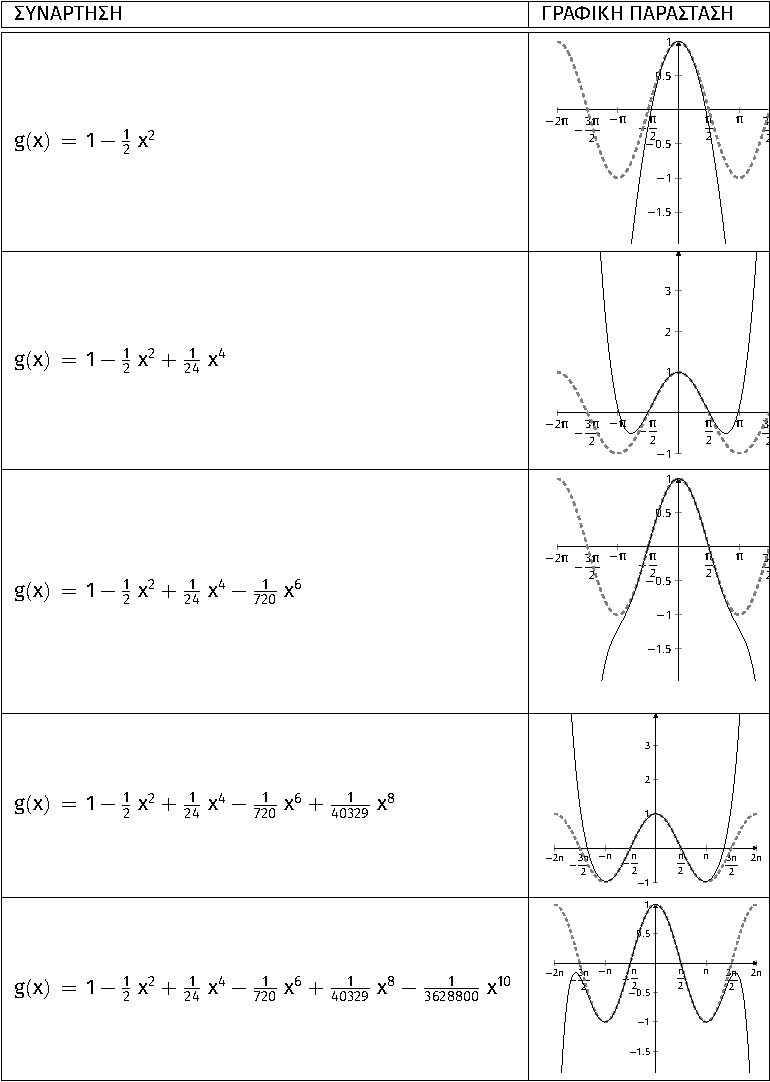
\includegraphics[width=0.99\textwidth]{tikzpic1.pdf}
	\caption{This is a picture}
\end{figure}
\begin{center}

	\textbf{"Γιατί η μελέτη των πολυωνύμων είναι σημαντική;"}.
\end{center}

Πέρα από τη χρησιμοθηρική προσέγγιση που αφορά τη συχνή τους χρήση στην επίλυση προβλημάτων στα πλαίσια του σχολείου και των Πανελλαδικών Εξετάσεων, θα παρουσιάσουμε μία εφαρμογή χρήσης των πολυωνύμων για την προσέγγιση άλλων\raisebox{0.4ex}{\em texhjkfh fhj kt} περισσότερο "δύσκολων συναρτήσεων."
\rule[4pt]{40pt}{1pt}
\begin{figure}[h]
	\centering	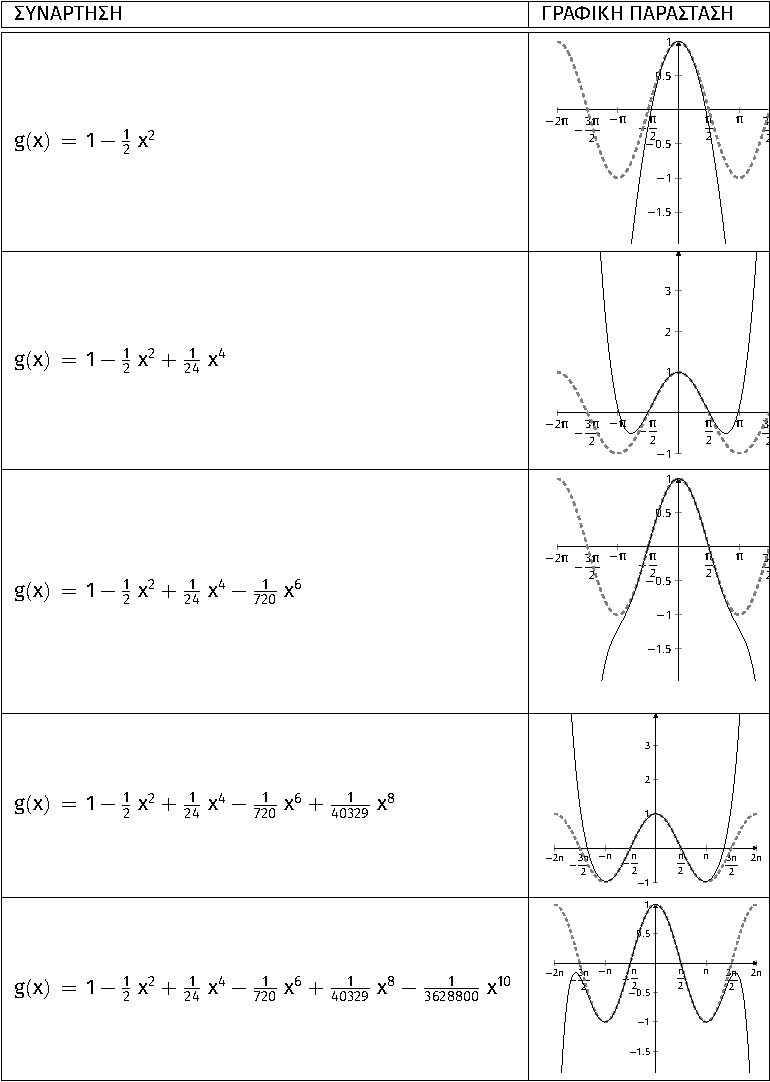
\includegraphics[width=0.99\textwidth]{tikzpic1.pdf}
\caption{This is a picture}
\end{figure}
\begin{figure}[h]
	\centering	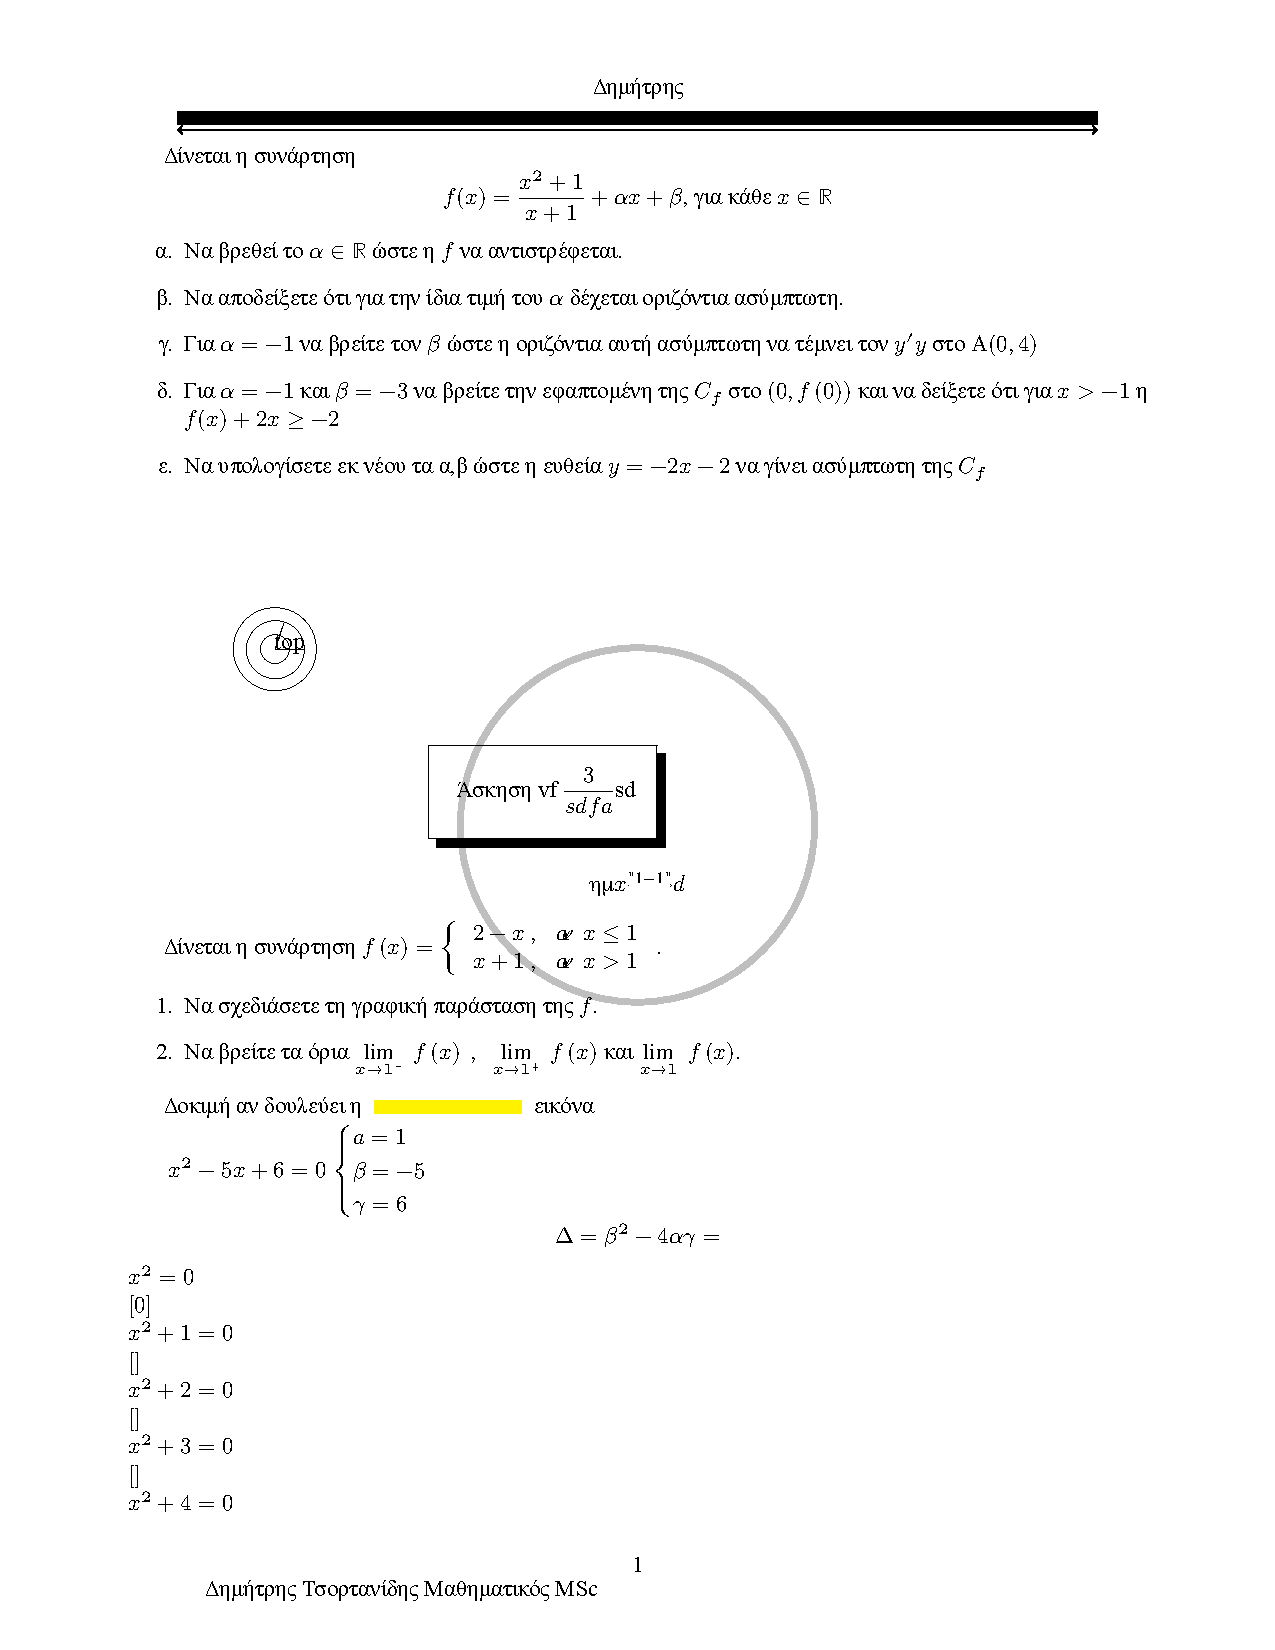
\includegraphics[width=0.5\textwidth]{askhshfb.pdf}
	\caption{This is a picture}
\end{figure}
\section*{Προσέγγιση του συνημιτόνου}
Στο Κεφάλαιο 2 της άλγεβρας συναντήσαμε την τριγωνομετρική συνάρτηση ${f(x)=συνx}$, την οποία μελετήσαμε ως προς την περίοδό της, τη μονοτονία της και τελικά με τη γραφική της παράσταση. Όποτε χρειάστηκε ο υπολογισμός της τιμής του συνημιτόνου μίας γωνίας, χρησιμοποιήθηκε είτε ο διαθέσιμος πίνακας τριγωνομετρικών αριθμών, ο οποίος βέβαια αναφέρεται στους \begin{figure}[h]
	\centering	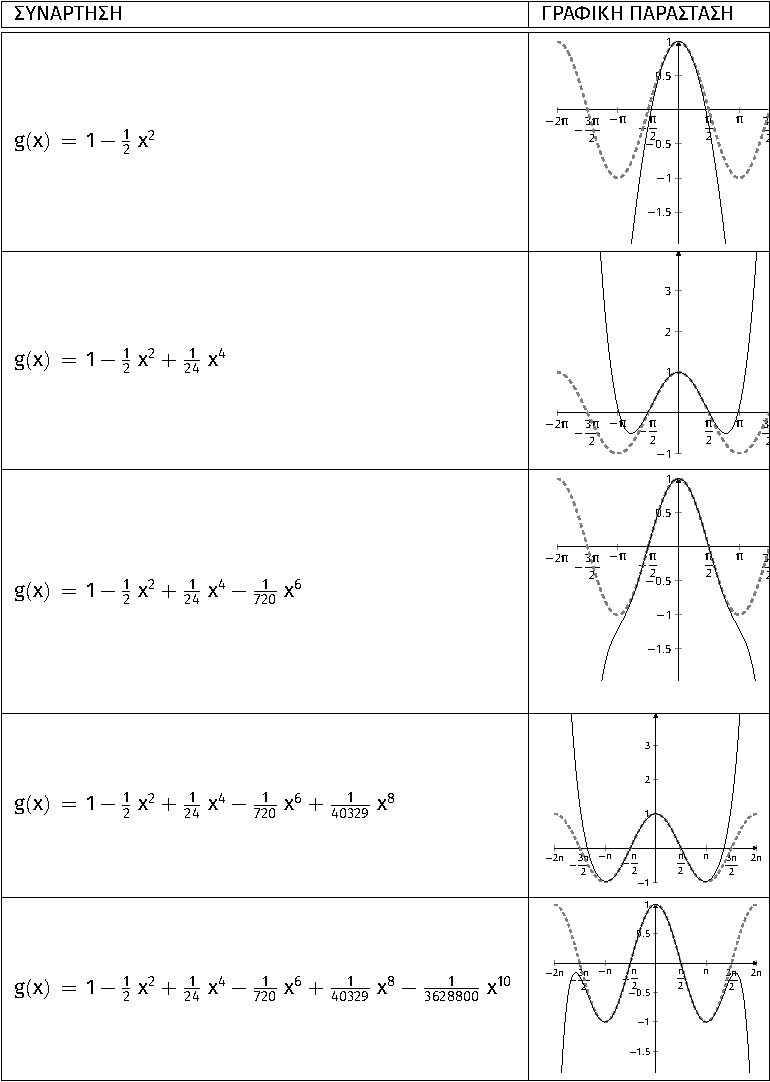
\includegraphics[width=0.99\textwidth]{tikzpic1.pdf}
	\caption{This is a picture}
\end{figure}τριγωνομετρικούς αριθμούς συγκεκριμένων γνωστών γωνιών, είτε χρησιμοποιήσαμε τις γνωστές τριγωνομετρικές ταυτότητες για το υπολογισμό ενός τριγωνομετρικού αριθμού εφόσον γνωρίζαμε κάποιον άλλο. Για παράδειγμα ο υπολογισμός των τριγωνομετρικών αριθμών της γωνίας $\dfrac{π}{16}$ από τους τριγωνομετρικούς αριθμούς της γνωστής γωνίας $\dfrac{π}{4}$ και τη χρήση των τριγωνομετρικών ταυτοτήτων των $ημ2α$,$συν2α$.
\begin{tabular}{||l|cr|}
\hline
1 & 2& 5\\\cline{2-3}
3 & 4&  \\\hline
\end{tabular}


		Δίνονται οι συναρτήσεις $f(x)=lnx,\mbox{ } x>0$ και $g(x)=\dfrac{x}{1-x}$, $x\neq 1$.
		\begin{enumerate}[label=\textbf{\roman*.}]
			\item{Να προσδιορίσετε τη συνάρτηση $f\circ g$}.\hfill \textbf{Μονάδες 5}
			
			\item Αν $h(x)=(f\circ g)(x)=ln\left(\dfrac{x}{1-x}\right)$,	$x\in(0,1) \mathbb{R} $, να αποδείξετε ότι η $h(x)$ είναι γνησίως αύξουσα και να βρείτε το σύνολο τιμών της.\\\strut \hfill \textbf{Μονάδες 7}
			
			
			
			\item  Να αποδείξετε ότι η συνάρτηση $h$ αντιστρέφεται και να βρείτε την αντίστροφή της. \\ \strut  \hfill \textbf{Μονάδες 6}
			
			
			\item Να βρείτε την εξίσωση της εφαπτομένης της $C_h$ στο σημείο τομής της με τον οριζόντιο  άξονα. \monades{7}
		\end{enumerate}



\end{document}
